\begin{center}
	\huge \textbf{Il modello PRNR}
	
	\rule{7cm}{0.4pt} 
	
	\LARGE Un modello matematico per la Rivoluzione Francese
	
	\vspace{20pt}
	
	\LARGE \textbf{Cristina Caprioglio, Luca Morelli}
	
	\vspace{5pt}
	
	\LARGE 20 Dicembre 2022
	
	\vspace{20pt}
 
	\normalsize
\end{center}  
\section*{Introduzione}
L'evoluzione di vari gruppi eterogenei all'interno di una popolazione può essere studiato sfruttando i modelli multicompartimentali. Questo tipo di modello matematico é ottimo per descrivere per esempio interazioni tra diverse specie in un ecosistema o la diffusione in una popolazione di un virus. Nel nostro caso, abbiamo utilizzato questo modello per studiare i meccanismi che portano allo scoppio di una rivoluzione e la sua soppressione. In particolare, abbiamo preso come sistema una popolazione con un elevato numero di individui che potevano, in base al loro reddito, appartenere o ai ricchi o ai nobili\footnote{Sul modello della tripartizione in stati dell'Ancien Regime.}, e abbiamo studiato in quali condizioni i primi potevano essere spinti a insorgere e i secondi a reprimere tali insurrezioni. Inoltre questa tipologia di modelli si adatta facilmente alla simulazione al calcolatore tramite l'impiego di automi cellulari, il che ci ha consentito di confrontare i risultati teorici con una simulazione.
\section{Il sistema e il modello} \label{sistema modello}
Come precedentemente detto, vogliamo studiare la dinamica di una popolazione composta da vari membri, in numero elevato, che differiscono l'uno dall'altro per il loro reddito. Queste differenze, sotto determinate condizioni, possono spingere gli individui appartenenti alla categoria più povera ad insorgere. Questa insurrezione può a sua volta portare alcuni tra i più abbienti a reprimerla con l'uso della forza.\\

Per modellizzare una popolazione eterogenea abbiamo deciso di suddividerla in due categorie, \textbf{Poveri} e \textbf{Nobili}, per le quali si considera un reddito medio caratteristico di ciascuna categoria.\\
Ogni membro di questa popolazione può decidere, in base a vari fattori, di far uso della violenza per far valere le esigenze del proprio gruppo. Abbiamo considerato che ogni individuo può trovarsi o in uno stato di normalità o in uno stato eccitato: un membro della categoria dei Poveri nello stato \textbf{Normale} $(N_P)$ può transire allo stato di \textbf{Rivoluzionario} $(R)$, mentre un membro della categoria dei Nobili nello stato \textbf{Normale} $(N_N)$ può transire allo stato di \textbf{Reazionario} $(\bar{R})$. All'interno della stessa categoria può avvenire anche la transizione inversa, come mostrato in figura \ref{fig:CompartmentScheme}.\\
\begin{figure}[H]
	\centering
	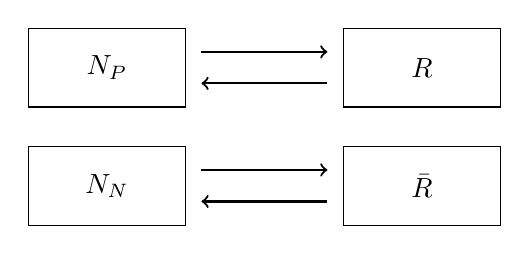
\begin{tikzpicture}
        \draw[draw=black] (0,0) rectangle (2,1);
		\draw[->, thick] (2.2,.7) -- (3.8,.7);
		\draw[<-, thick] (2.2,.3) -- (3.8,.3);
		\draw[draw=black] (4,0) rectangle (6,1) ;
		\node at (5,0.5) {$\bar{R}$};
		\node at (1,0.5) {$N_N$};
		\draw[draw=black] (0,1.5) rectangle (2,2.5);
		\draw[->, thick] (2.2,2.2) -- (3.8,2.2);
		\draw[<-, thick] (2.2,1.8) -- (3.8,1.8);
		\draw[draw=black] (4,1.5) rectangle (6,2.5) ;
		\node at (5,2) {$R$};
		\node at (1,2) {$N_P$};
    \end{tikzpicture}
	
	\caption{Schema a compartimenti delle categorie delle persone. Con le frecce sono evidenziate le transizioni di stato che un individuo può effettuare.}\label{fig:CompartmentScheme}
\end{figure}
Per questa modellizazione abbiamo deciso, come è consueto fare, di trascurare le possibili fluttuazioni del numero totale di individui dovuti alla morte e alla nascita di persone, inoltre abbiamo considerato che un individuo non possa transire dalla categoria di Povero a quella di Nobile. Questa scelta è giustificata dall'osservazione che, seppur possibili, tali transizioni in genere sono estremamente rare. Tali considerazioni ci hanno quindi permesso di identificare 3 vincoli da imporre al modello:
\begin{equation}
    \frac{N_P(t)+R(t)}{N_P(0)+R(0)+N_N(0)+\bar{R}(0)}=F_P \quad\:\frac{N_N(t)+\bar{R}(t)}{N_P(0)+R(0)+N_N(0)+\bar{R}(0)}=F_N \quad\: F_P+F_N=1 
	\label{vincoli}
\end{equation}
dove $F_P$ e $F_N$ sono rispettivamente le frazioni di individui Poveri e Nobili sulla popolazione totale.\\

Dobbiamo ora identificare quali equazioni regolino la dinamica del sistema. Per fare ciò abbiamo ragionevolmente supposto che:
\begin{itemize}
	\item un Povero possa transire allo stato di Rivoluzionario o di sua spontanea iniziativa (dovuta alla sua condizione disagiata) oppure incontrando un rivoluzionario che lo convinca ad insorgere;
	\item un Rivoluzionario, incontrando dei Reazionari, possa essere convinto a non perseguire più la sua causa ritornando allo stato Normale;
	\item un Nobile, incontrando un rivoluzionario, possa in risposta decidere di diventare un Reazionario;
	\item un Reazionario, vedendo diminuire il numero di Rivoluzionari (e quindi aumentare quello di Poveri allo stato normale), possa decidere di ritornare anch'esso allo stato normale.
\end{itemize}
Se consideriamo un tempo $\Delta t$ possiamo esprimere le variazioni del numero di ogni compartimento, tenendo conto delle precedenti considerazioni, con:

\begin{equation}\label{modelloDiscreto}
	\begin{aligned}
		 &R(t+\Delta t)-R(t)=\Gamma N_P(t) \frac{R(t)}{N_{tot}}\Delta t+\gamma N_P(t)\Delta t-\bar{\Gamma}R(t)\frac{\bar{R}(t)}{N_{tot}}\Delta t\\
		&\bar{R}(t+\Delta t)-\bar{R}(t)=\alpha N_N(t)\frac{R(t)}{N_{tot}}\Delta t-\beta \bar{R}(t)\frac{N_P(t)}{N_{tot}}\Delta t\\
		&N_P(t+\Delta t)-N_P(t)=-(R(t+\Delta t)-R(t))\\
		&N_N(t+\Delta t)-N_N(t)=-(\bar{R}(t+\Delta t)-\bar{R}(t))\\
	\end{aligned}     
\end{equation}	
dove $ \Gamma $ é un parametro che stima la probabilità che un povero diventi rivoluzionario incontrando altri rivoluzionari, mentre invece $ \bar{\Gamma} $ stima la probabilità che un rivoluzionario ritorni allo stato Normale.  Diversamente dai precedenti parametri $\gamma$ stima la probabilità che un povero diventi rivoluzionario per volontà propria. Infine $ \alpha $ e $ \beta $ sono i due parametri relativi alla variazione dei reazionari: il primo riguarda la probabilità che un nobile diventi reazionario mentre il secondo che un reazionario torni allo stato Normale. \\
Ogni parametro è quindi moltiplicato per la probabilità che il singolo individuo ne incontri un secondo che possa indurlo a transire (per esempio un povero incontra un rivoluzionario), questa probabilità è stimata dalla frazione dei secondi sulla popolazione totale. Per ottenere il numero di individui che transiscono è quindi necessario moltiplicare questa probabilità per il numero di persone che potenzialmente possono effettuare la transizione. Infine è opportuno osservare che queste probabilità sono stimate per unità di tempo, quindi ogni addendo va moltiplicato per $\Delta t$, così da ottenere le variazioni di popolazione per ogni compartimento nel tempo $\Delta t$.\\


Si osservi che, riscalando di un fattore $\lambda$ tutta la popolazione, le equazioni (\ref{modelloDiscreto}) non mutano forma. Questo ci ha permesso di riscalare le variabili dividendole per $ N_{tot}$, che indica la popolazione totale. In questo modo otteniamo un sistema di equazioni che esprime come variano le frazioni di ogni categoria di persone sulla popolazione totale:  

\begin{equation} \label{eq: 1.3}
	\begin{aligned}
		&R'(t+\Delta t)-R'(t)=\Gamma N'_P(t)'R'(t)\Delta t+\gamma N'_P(t)\Delta t-\bar{\Gamma}R'(t)\bar{R'}(t)\Delta t\\
	&\bar{R'}(t+\Delta t)-\bar{R'}(t)=\alpha N'_N(t)R'(t)\Delta t-\beta \bar{R'}(t)N'_P(t)\Delta t\\
	&N'_P(t+\Delta t)-N'_P(t)=-(R'(t+\Delta t)-R'(t))\\
	&N'_N(t+\Delta t)-N'_N(t)=-(\bar{R'}(t+\Delta t)-\bar{R'}(t))\\
	\end{aligned}
\end{equation}	
con 
\begin{equation*}
	N'_{P}(t)=\frac{N_{P}(t)}{N_{tot}} \qquad 	N'_{N}(t)=\frac{N_{N}(t)}{N_{tot}} \qquad	R'(t)=\frac{R(t)}{N_{tot}} \qquad	\bar{R'}(t)=\frac{\bar{R}(t)}{N_{tot}} 
\end{equation*}
Per alleggerire la notazione, dato che da questo momento in poi useremo spesso le variabili riscalate, quest'ultime perderanno il simbolo ``$ ' $" e verranno scritte normalmente, indicheremo quindi quando queste vadano intese senza normalizzazione. \\
%
%All'interno della simulazione, visto che si calcolava la probabilità di ogni singolo individuo di compiere una transizione e non la variazione nel tempo dell'intero settore, tutti i parametri (con l'eccezione di $ \gamma $) sono stati divisi per 8. Questo perchè, calcolando la probabilità che avvenga una transizione, se la prima è influenzata dalla presenza o meno di un membro appartenente ad una certa categoria, andrà moltiplicata per la probabilità di incontrarlo. Nel nostro caso, ogni persona poteva interagire solo con le 8 celle adiacenti, perciò abbiamo dovuto moltiplicare per $ \frac{1}{8} $.
%\textbf{(NON SAREBBE MEGLIO METTERLO DOPO?)}
\\
Per poter studiare il nostro modello abbiamo diviso ogni espressione per $ \Delta t $ e, considerando intervalli di tempo abbastanza piccoli, abbiamo ottenuto un sistema di equazioni differenziali tramite il passaggio al continuo:
\begin{equation} \label{eq:1.4}
		\begin{aligned}
			&\frac{dR}{dt}=\Gamma N_P(t) R(t)+\gamma N_P(t)-\bar{\Gamma}R(t)\bar{R}(t)\\
		&\frac{d\bar{R}}{dt}=\alpha N_N(t)R(t)-\beta \bar{R}(t)N_P(t)\\
		&\frac{dN_{P}}{dt}= -\frac{dR}{dt}\\
		&\frac{dN_{R}}{dt}= -\frac{d\bar{R}}{dt}\\
		\end{aligned}
\end{equation}
Abbiamo quindi studiato il comportamento generale di queste equazioni per caratterizzare il modello.
\subsection{Punti di equilibrio}
Come primo passo abbiamo studiato i punti di equilibrio del sistema: ricordando i vincoli (\ref{vincoli}), ossia per la popolazione normalizzata $
	F_{P}=N_{P}+R ,\ F_{N}=N_{N}+\bar{R}
$, e ponendo uguali a zero le derivate prime delle equazioni (\ref{eq:1.4}) abbiamo ottenuto un sistema che consente di determinare i punti cercati:
\begin{equation}
	\begin{cases}
		\Gamma (F_{P}-R)R+\gamma (F_{P}-R)-\bar{\Gamma}R\bar{R}=0\\
		\alpha (F_{N}-\bar{R})R-\beta (F_{P}-R)\bar{R}=0
	\end{cases}
\end{equation}La (1.5) rappresenta l'intersezione di due iperboli, a meno che $\alpha=\beta$ per cui un'iperbole degenera in una retta.
Eseguendo alcuni passaggi algebrici\footnote{Per tutti i passaggi si veda l'appendice B} si può ottenere $ \bar{R} $ in funzione di $ R $ e sostituendolo nella seconda equazione del sistema otteniamo la seguente equazione di terzo grado:
\begin{equation}
	R^{3}(\beta - \alpha)\frac{\Gamma}{\bar{\Gamma}}-R^{2}\left(\alpha F_{N}+(\beta - \alpha)\frac{\Gamma}{\bar{\Gamma}}F_{P}-(\beta - \alpha)\frac{\gamma}{\bar{\Gamma}}+\beta F_{P}\frac{\Gamma}{\bar{\Gamma}}\right)-\frac{R}{\bar{\Gamma}}\left(\gamma (\beta - \alpha)F_{P}-\beta \Gamma F^{2}_{P}+\gamma\beta F_{P}\right)+\frac{\gamma\beta}{\bar{\Gamma}}F^{2}_{P}
	\label{equilibiro 3g}=0
\end{equation}
Le soluzioni della (\ref{equilibiro 3g}) devono però essere valori compresi tra $0$ e $1$ poichè abbiamo normalizzato la popolazione. \'{E} facile dimostrare che il polinomio \ref{equilibiro 3g} ha almeno uno zero nell'intervallo $ \left[0,1\right] $: infatti per $ R=0 $ si riduce a
\begin{equation}
	\frac{\gamma\beta}{\bar{\Gamma}}F^{2}_{P}\geq0\qquad \forall \gamma, \beta, \bar{\Gamma}, F_{P}
\end{equation}
mentre per $ R=1 $ otteniamo
\begin{equation}
	-\alpha F_{N}\left[1+\frac{\Gamma+ \gamma}{\bar{\Gamma}}\right]\leq0\qquad \forall \gamma, \alpha, \Gamma, \bar{\Gamma}, F_{N}.
\end{equation}
Per il teorema degli zeri, dato che la funzione assume valori di segno opposto agli estremi dell'intervallo, deve annullarsi in almeno un punto appartenente all'intervallo. Inoltre possiamo evincere che $R=0$ è un punto di equilibrio solo se $\gamma$ o $\beta$ o $F_P$ sono nulli, analogamente $R=1$ è un punto di equilibrio solo se $\alpha$ o $F_N$ sono identicamente nulli. Quest'ultima osservazione non stupisce, infatti in entrambi i casi o la popolazione è composta di una sola categoria di persone, perdendo così di senso, oppure i parametri che stimano la probabilità di insorgere per ogni categoria devono annullarsi.
\\
Per ogni set di parametri abbiamo quindi determinato i punti di equilibrio e ottenuti questi ci è stato possibile studiare in un intorno di tali punti la stabilità del sistema: detti $R_{eq},\ \bar{R}_{eq}$ rispettivamente il numero di rivoluzionari e reazionari all'equilibrio e studiando $\delta R(t)=R(t)- R_{eq}$ e $\delta \bar{R}(t)=\bar{R}(t)-\bar R_{eq}$ nel sistema linearizzato si ottiene:
\begin{equation}
	\begin{pmatrix}
		\delta \dot{R}\\ 
		\delta \dot{\bar{R}}
	\end{pmatrix}
	=\begin{pmatrix}
		\Gamma(F_P-2R_{eq})-\gamma-\bar{\Gamma} \bar{R}_{eq} & -\bar{\Gamma}R_{eq}\\
		\alpha(F_{N}-\bar{R}_{eq})+\beta \bar{R}_{eq} & -\alpha R_{eq}+\beta R_{eq}
	\end{pmatrix}
	\begin{pmatrix}
		\delta R\\
		\delta \bar{R}
	\end{pmatrix}
\end{equation} 
che abbiamo utilizzato per studiare il tipo di equilibrio del sistema. Nella fattispecie è necessario che la matrice del sistema linearizzato sia definita negativa affinché il punto di equilibrio sia stabile.\\
Per esempio abbiamo già mostrato che $R=0$ può essere un punto di equilibrio: in tal caso dalla (1.5) si ha che $F_P$ deve essere nullo e $\bar R_{eq}$ può assumere qualsiasi valore in $[0,1]$. In questo caso l'equilibrio risulta stabile, ma come abbiamo osservato questo si verifica solo se non vi sono poveri.\\
%aggiungere conti che ho fatto
\section{Integrazione}
Le equazioni (\ref{eq:1.4}) che abbiamo descritto nella sezione \emph{\ref{sistema modello}} non sono facilmente risolvibili, per questo motivo può essere opportuno integrarle numericamente. Il metodo utilizzato per l'integrazione é quello di Runge-Kutta al quarto ordine, il quale permette di approssimare una funzione conoscendone la derivata prima rispetto al tempo e le condizioni iniziali\footnote{Per una spiegazione dettagliata si veda l'appendice A}. \\
Considerando come unità di tempo i giorni e utilizzando un passo di integrazione di $ h=0.01 \text{ giorni}$ siamo riusciti ad ottenere l'andamento di $ N_{P}, N_{N}, R$ e $\bar{R} $ nel tempo secondo le equazioni (\ref{eq:1.4}) per diversi valori iniziali e paramenti di simulazione.
\begin{figure}[H]
	\centering
	\begin{subfigure}[H]{0.49\textwidth}
		\centering
		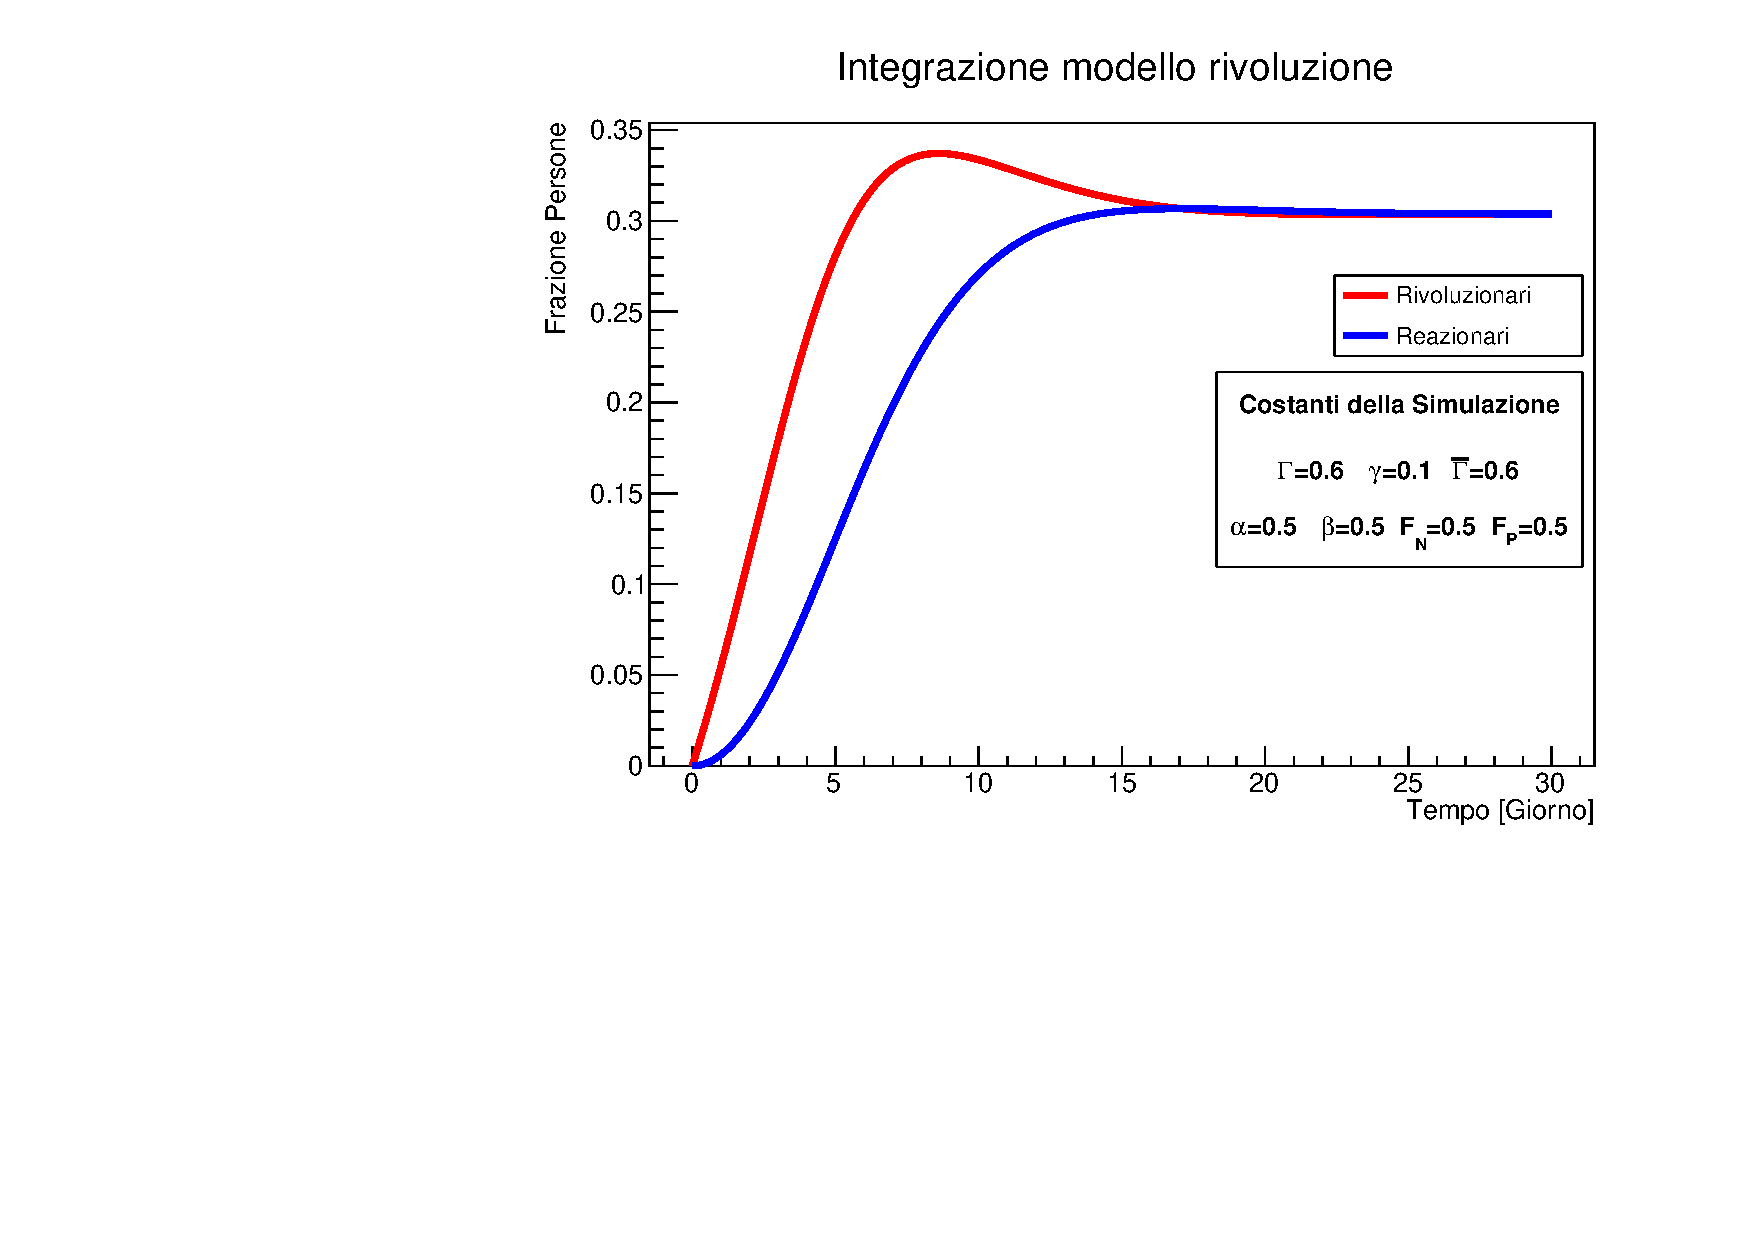
\includegraphics[width=\textwidth]{COMPENSATO.pdf}
	\end{subfigure}
	\hfill
	\begin{subfigure}[H]{0.49\textwidth}
		\centering
		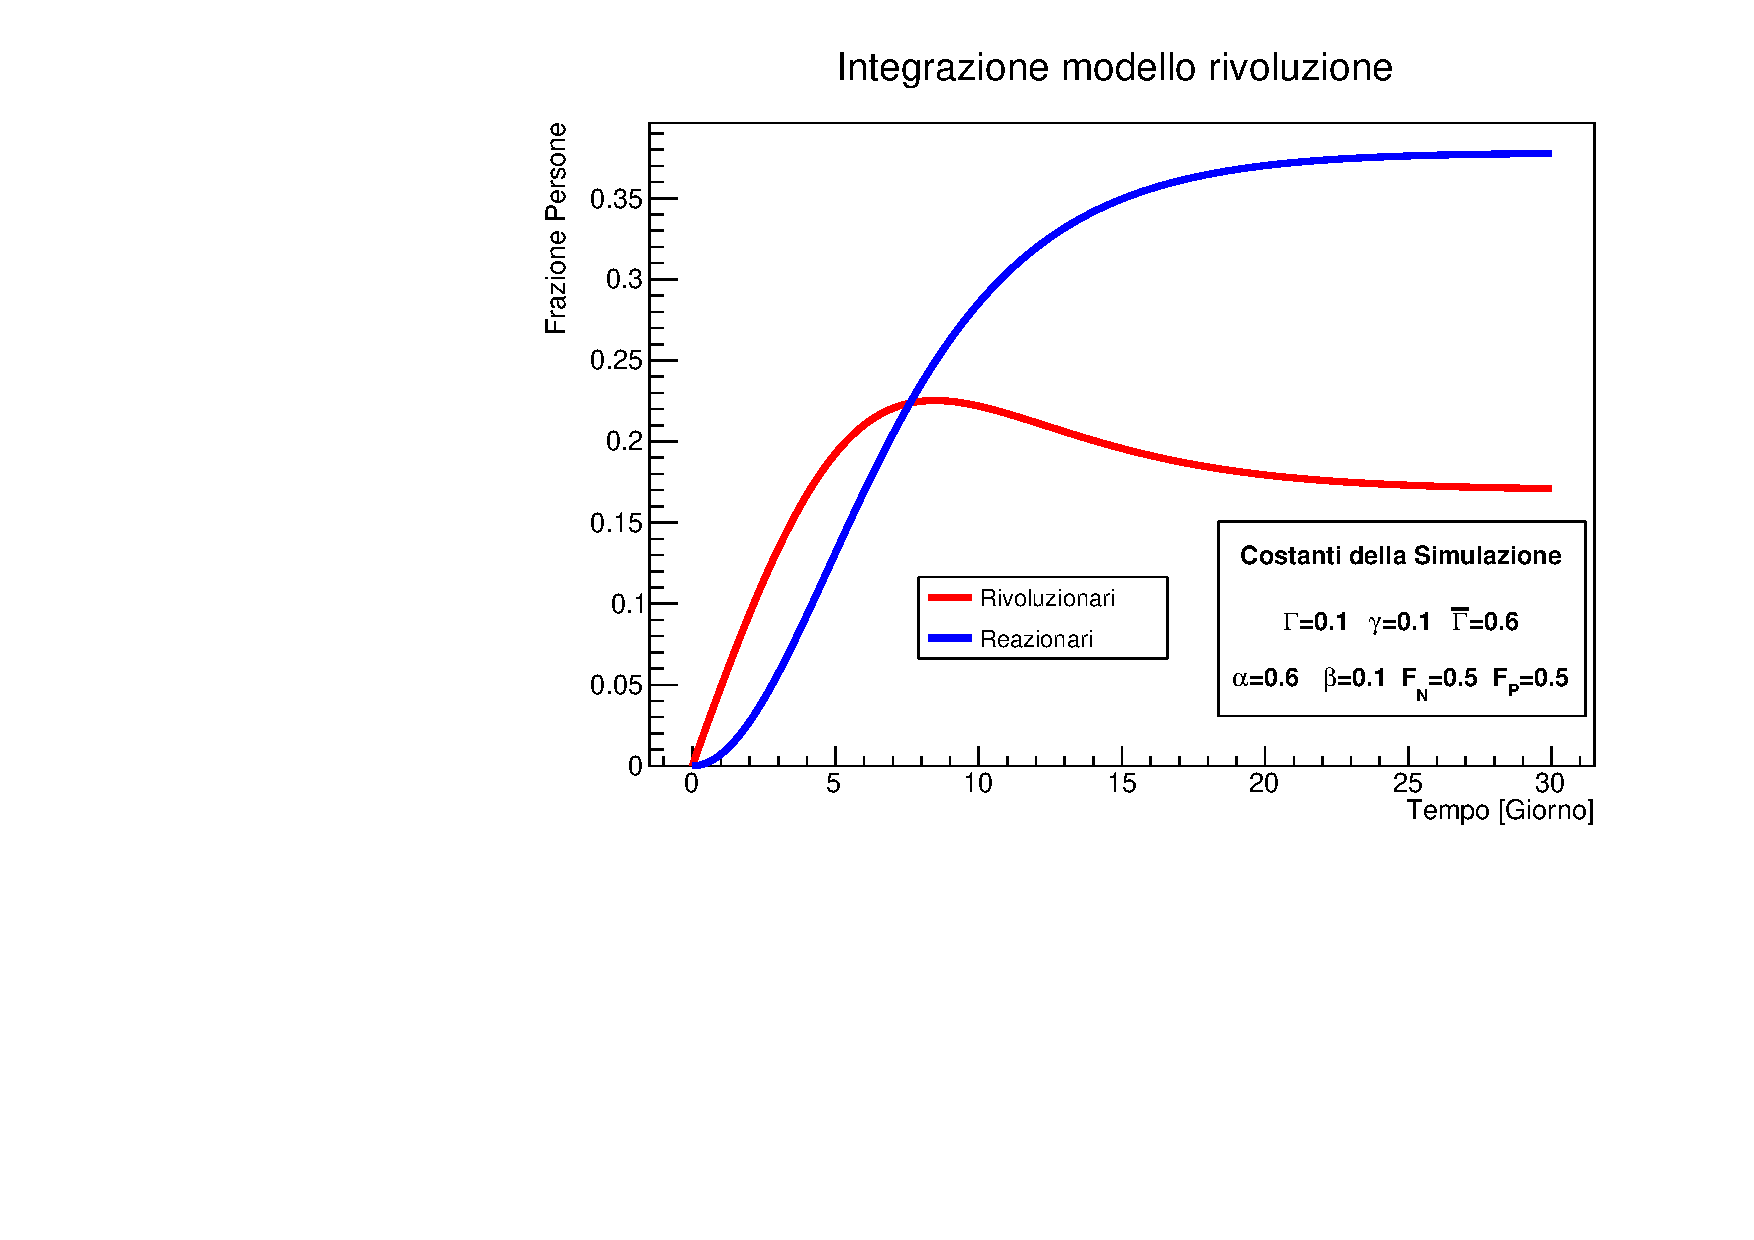
\includegraphics[width=\textwidth]{FORZARICCHI.pdf}
	\end{subfigure}
\caption{Due esempi di integrazione del modello}
\label{grafici integrazione}
\end{figure}
Nei grafici in Fig.\ref{grafici integrazione} si può apprezzare lo scoppio della rivoluzione seguito dalla risposta dei nobili. Infatti il punto $R=0,\ \bar{R}=0$ costituisce un punto dove, per termine contenente $\gamma$, ha origine una iniziale crescita esponenziale. L'iniziale crescita esponenziale genera, nella maggior parte dei casi, un picco di rivoluzionari che scema leggermente con la risposta dei reazionari. Nel primo grafico i due gruppi tendono a due punti di equilibrio vicini, questo poiché sono stati scelti parametri tali da bilanciare le due categorie, nel secondo grafico invece il numero di reazionari supera quello di rivoluzionari mantenendo quest'ultimo basso.
\section{Simulazione}
Per verificare la validità del modello matematico appena descritto abbiamo deciso di effettuare una simulazione al calcolatore di una dinamica di popolazione. Le equazioni (\ref{modelloDiscreto}), per la loro natura discreta, si adattano molto bene al modello dell'automa cellulare: una popolazione è rappresentata in questo modello da una griglia di celle, ognuna corrispondente ad un individuo che può trovarsi in un determinato stato.
\begin{center}
	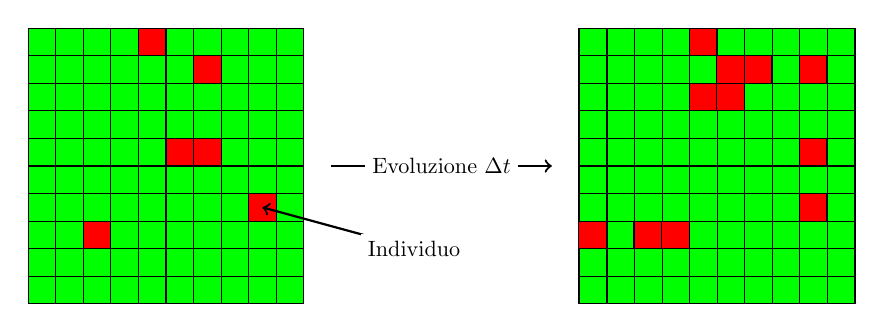
\begin{tikzpicture}[scale=0.7]
		\draw[fill=green] (0,0) rectangle (5,5);
		\draw[fill=green] (9.99,0) rectangle (15,5);
		\draw[step=0.5cm] (0,0) grid (5,5);
		\draw[step=0.5cm] (9.99,0) grid (15,5);
		
		\filldraw[fill=red] (1,1) rectangle (1.5,1.5);
		\filldraw[fill=red] (3,4) rectangle (3.5,4.5);
		\filldraw[fill=red] (4,1.5) rectangle (4.5,2);
		\filldraw[fill=red] (2,4.5) rectangle (2.5,5);
		\filldraw[fill=red] (2.5,2.5) rectangle (3,3);
		\filldraw[fill=red] (3,2.5) rectangle (3.5,3);
		
		\draw[->,thick] (5.5,2.5) -- (9.5,2.5);
		\node[fill=white,scale=0.8] at (7.5,2.5) {Evoluzione $\Delta t$};
		
		\filldraw[fill=red] (10.99,1) rectangle (11.49,1.5);
		\filldraw[fill=red] (12.99,4) rectangle (13.49,4.5);
		\filldraw[fill=red] (13.99,1.5) rectangle (14.49,2);
		\filldraw[fill=red] (11.99,4.5) rectangle (12.49,5);
		\filldraw[fill=red] (12.49,4) rectangle (12.99,4.5);
		\filldraw[fill=red] (11.49,1) rectangle (11.99,1.5);
		\filldraw[fill=red] (9.99,1) rectangle (10.49,1.5);
		\filldraw[fill=red] (13.99,4) rectangle (14.49,4.5);
		\filldraw[fill=red] (13.99,2.5) rectangle (14.49,3);
		\filldraw[fill=red] (11.99,3.5) rectangle (12.49,4);
		\filldraw[fill=red] (12.49,3.5) rectangle (12.99,4);
		\filldraw[fill=red] (10.99,1) rectangle (11.49,1.5);
		
		\draw[<-,thick] (4.25,1.75) -- (7,1);
		\node[fill=white,scale=0.8] at (7,1) {Individuo};
	\end{tikzpicture}
\end{center}
La simulazione che abbiamo realizzato fa variare lo stato di ogni cella secondo le equazioni (\ref{modelloDiscreto}) ad intervalli di tempo discreto $\Delta t$ e ogni cella interagisce con quelle adiacenti\footnote{Nel nostro caso ogni cella ha 8 celle adiacenti che vengono considerate.} simulando l'incontro con altri individui. Così facendo, per ogni individuo che può indurre una transizione di stato, viene probabilisticamente determinato se questa debba aver luogo o meno e si modifica quindi lo stato della cella. Il carattere probabilistico è determinato dai parametri $\Gamma,\ \bar{\Gamma},\ \gamma,\ \alpha $ e $\beta$, è stato però necessario tener conto delle limitazioni della simulazione, infatti una cella può realmente interagire solamente con le otto adiacenti e non con tutta la popolazione, per questo le probabilità di transizione nelle equazioni (\ref{modelloDiscreto}) sono state riscalate di un fattore $\frac{1}{8}$ quando utilizzate nella simulazione.  \\ 
I risultati che abbiamo così ottenuto possono essere paragonati a quelli ottenuti tramite l'integrazione del modello. Questo confronto è esemplificato nei grafici \ref{confromto} nei quali sono riportati sia i risultati della simulazione che quelli dell'integrazione per lo stesso set di parametri.\\ 
\begin{figure}[H]
	\centering
	\begin{subfigure}[H]{0.49\textwidth}
		\centering
		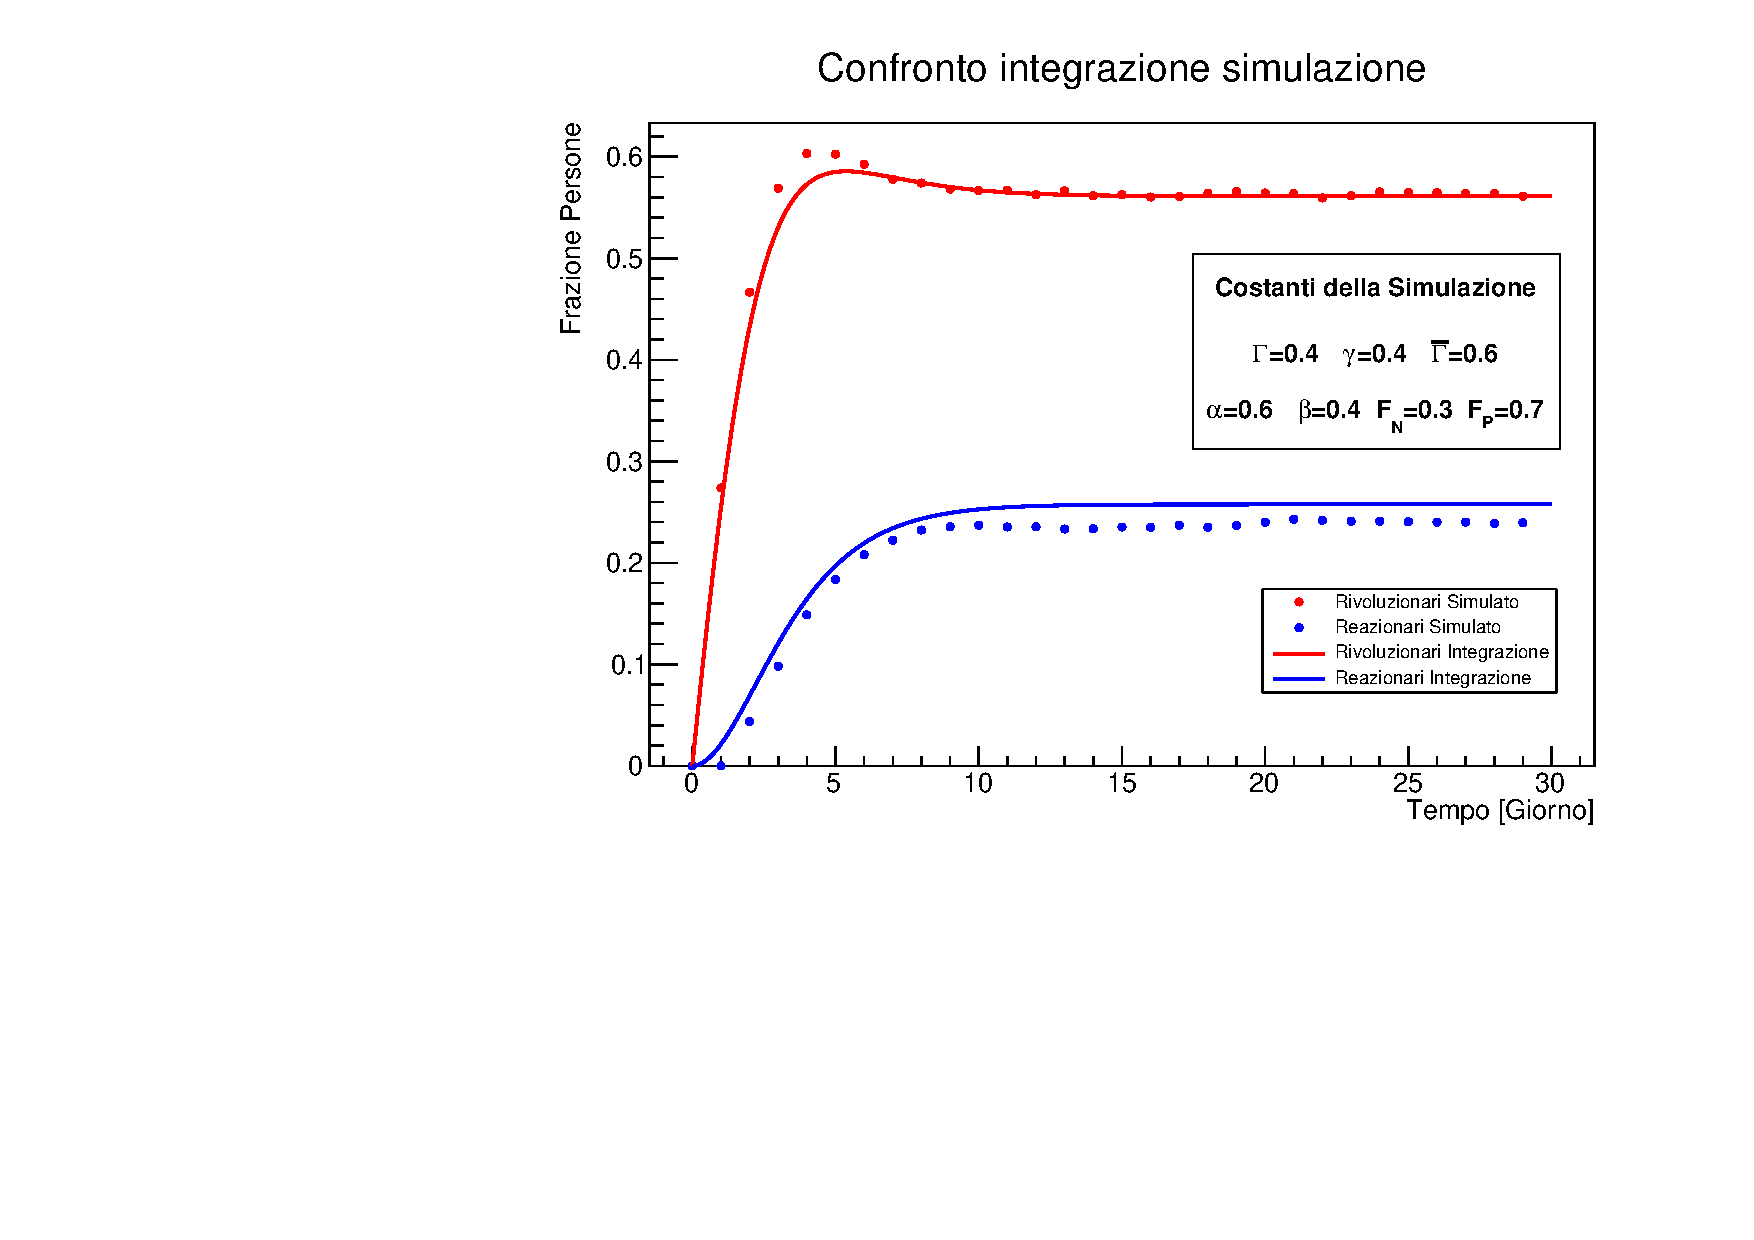
\includegraphics[width=\textwidth]{CONFRONTO1.pdf}
	\end{subfigure}
	\hfill
	\begin{subfigure}[H]{0.49\textwidth}
		\centering
		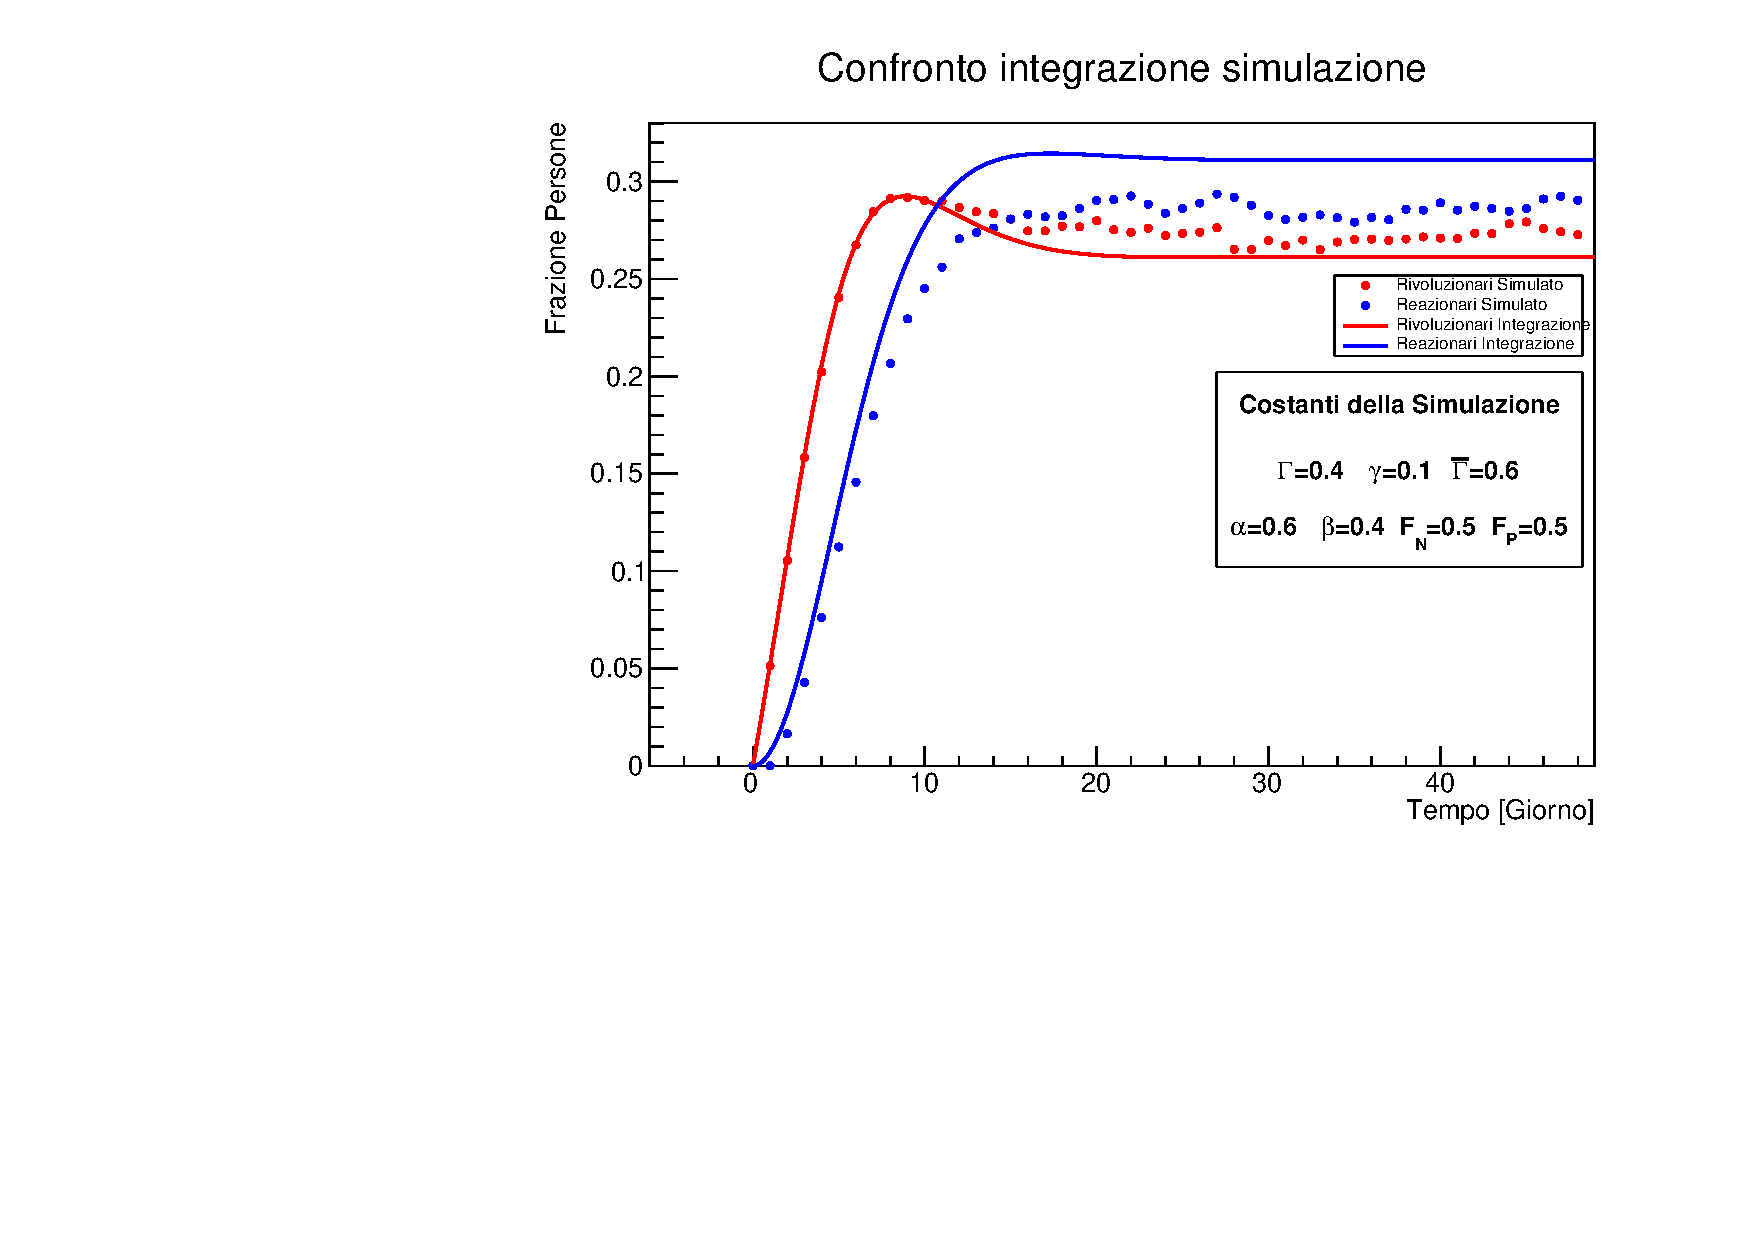
\includegraphics[width=\textwidth]{Confronto2.pdf}
	\end{subfigure}
	\caption{Due esempi di confronto tra simulazione ed integrazione}
	\label{confromto}
\end{figure}
Come si può notare i risultati sono in accordo tra loro, soprattutto nel periodo transiente. Nel secondo grafico si può notare infatti come nella fase costante ci siano delle fluttuazioni nei dati simulati, questo è dovuto essenzialmente alla natura stocastica della simulazione che non riesce quindi a generare veri e propri punti di equilibrio, ma oscilla attorno ad essi. In ogni caso, considerando la natura della simulazione, possiamo affermare che il modello matematico che abbiamo descritto costituisce una buona descrizione di una dinamica d'interazione sociale.
\section{Modulazione dei parametri}
Al fine di rendere il modello più realistico abbiamo deciso di rendere variabili i parametri relativi alla variazione dei rivoluzionari. Per prima cosa abbiamo definito una funzione che stima la differenza media di ricchezza posseduta tra un nobile e un povero: $\Delta\text{Pil}$. Questa ha una dipendenza temporale che può quindi influenzare lo stato della popolazione, simulando vari scenari come periodi di carestie o interventi sociali da parte dello stato.\\
Inoltre abbiamo introdotto un paramento $\sigma$ che misura la suscettibilità dei poveri alle loro condizioni economiche nell'ambiente sociale; nella fattispecie questo tiene conto di come pochi poveri non saranno molto propensi all'insurrezione mentre se è la maggior parte della popolazione a trovarsi in condizione di povertà tale evento è più facile che si verifichi. Abbiamo assunto che tale parametro sia stimato dalla seguente funzione: 
\begin{equation}
	\sigma= \sigma_0\left(1-\exp\left\{-\frac{F_P}{F_N}\right\}\right)
\end{equation}
questa infatti tende a $0$ per $F_P$ che tende a $0$ e a $\sigma_0$ per $F_N$ che tende a $0$.\\
Alla luce di queste considerazioni le probabilità di transizione diventano dipendenti da $\sigma$ e $\Delta\text{Pil}$:
\begin{equation}
	\begin{aligned}
	&\Gamma=\Gamma_{0}\cdot\tanh\left(\sigma\cdot \Delta\text{Pil}\right)\\
	&\gamma=\gamma_{0}\cdot\tanh\left(\sigma\cdot \Delta\text{Pil}\right)\\
	&\bar{\Gamma}=\bar{\Gamma}_{0}\cdot\tanh\left(\frac{1}{\sigma\cdot \Delta\text{Pil}}\right)\\
	\end{aligned}
\end{equation}
con questi andamenti funzionali abbiamo voluto tener conto di come la probabilità di transire in uno stato di insurrezione di un individuo sia massima quando le condizioni di povertà diventano estreme per buona parte della popolazione, infatti la tangente iperbolica funge da funzione di soglia che risulta poco sensibile a piccoli valori del suo argomento mentre invece cresce rapidamente ad $1$ per valori più grandi. Il parametro $\sigma$ invece varia proprio questa sensibilità della funzione $\tanh$.\\
Di seguito sono elencati i tre tipi diversi di funzioni $ \Delta Pil $ che abbiamo utilizzato e i relativi grafici:
\begin{itemize}
	\item \textbf{Carestie periodiche}\\
\begin{equation}
	\Delta\text{Pil}(t)=
	\begin{cases}
		\Delta\text{Pil}_0\sin(2\pi\nu t)\qquad \text{Se $ \sin(2\pi\nu t)>0 $} \qquad (\nu=\text{Frequenza carestia }) \\
		0 \qquad \qquad\qquad \qquad \,\text{Altrimenti}
	\end{cases}
\end{equation}
\begin{figure}[H]
	\centering
	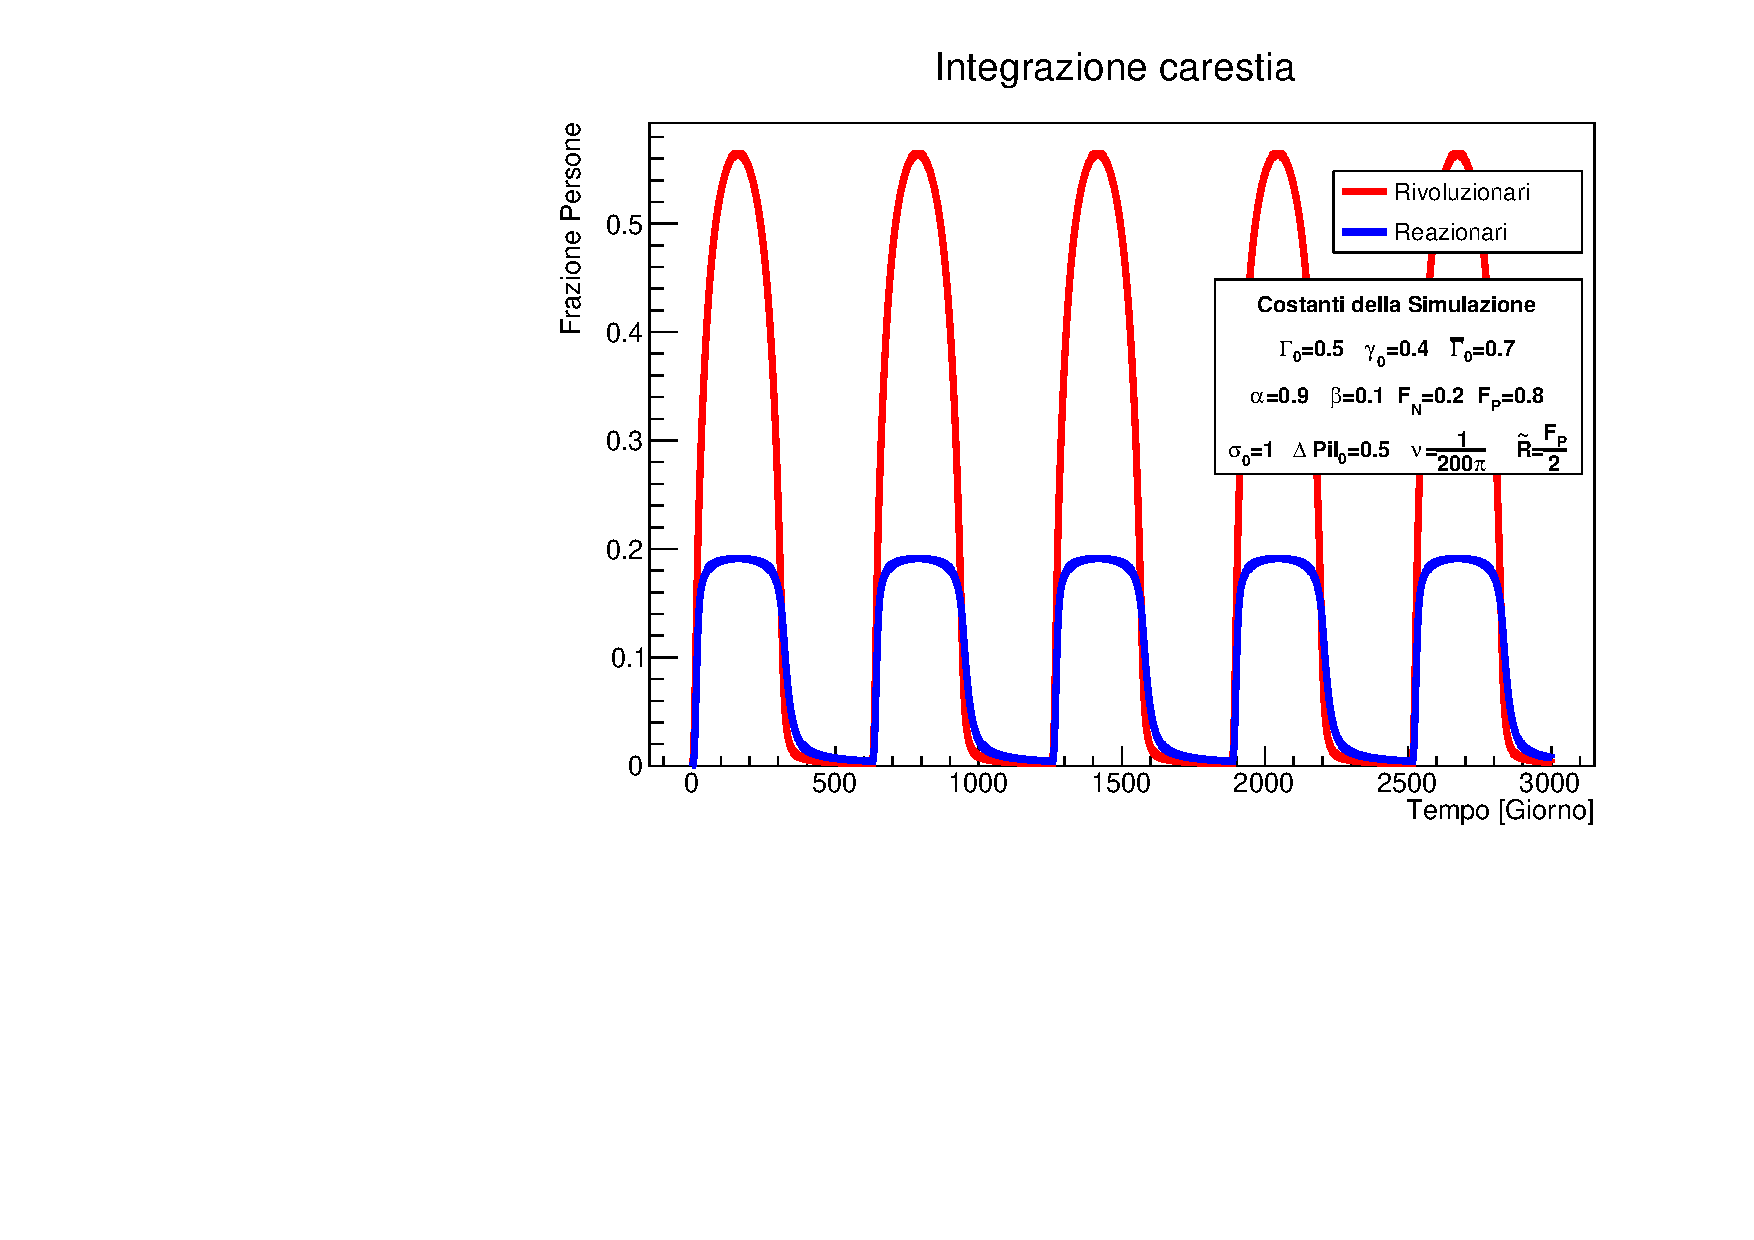
\includegraphics[scale=0.4]{SIN.pdf}
	\caption{Integrazione del modello con simulazione di carestie periodiche.}
\end{figure}
Abbiamo fatto variare il parametro della povertà secondo una sinusoide solamente positiva così da simulare brevi periodi di carestie in cui la povertà cresce per poi annullarsi per brevi periodi: in questo modo il modello manifesta tante rivolte che scemano nel momento in cui la carestia cessa.\\
\item \textbf{Sussidi statali}\\
\begin{equation}
	\Delta\text{Pil}(t)=
	\begin{cases}
		\Delta\text{Pil}_0 \qquad \quad \text{Se $R(t)$ non è mai salito oltre un livello soglia $\tilde{R}$}\\
		\Delta\text{Pil}_0\ e^{-\frac{t}{\lambda}} \quad \text{Altrimenti}\qquad     \text{($\lambda=$Rapidità intervento)}
	\end{cases}
\end{equation}
\begin{figure}[H]
	\centering
	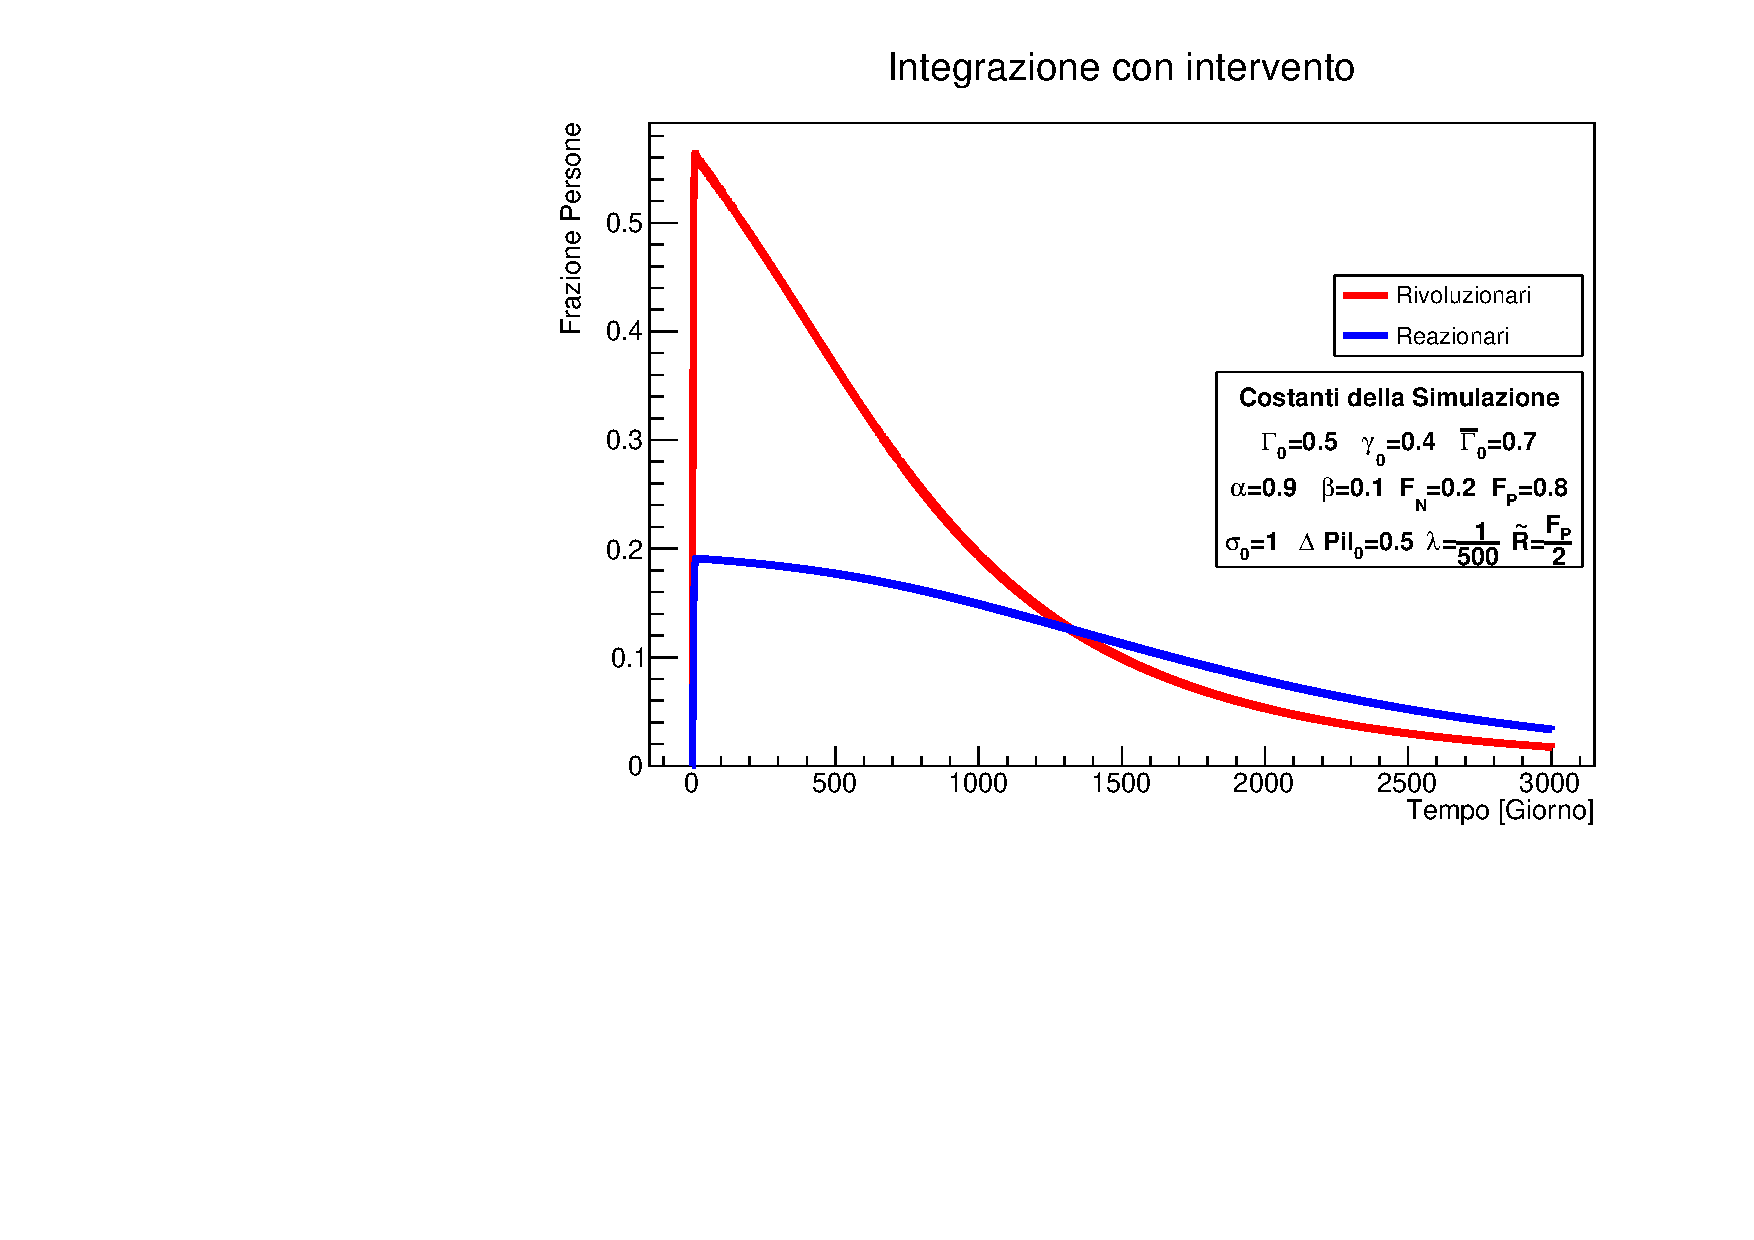
\includegraphics[scale=0.4]{EXP.pdf}
	\caption{Integrazione del modello con simulazione di interventi esterni.}
\end{figure}
In questo caso abbiamo integrato il modello richiedendo che, superato un certo parametro di soglia, vi fosse un intervento esterno atto a diminuire la povertà così da controllare la rivoluzione. Questo tipo di interazione riesce nel suo scopo facendo decrescere il numero di rivoluzionari fino ad un punto nel quale il numero di questi scende sotto a quello dei reazionari ponendo così fine alla rivolta.
\item \textbf{Carestie con sussidi}
\begin{equation}
	\Delta\text{Pil}(t)=
	\begin{cases}
		0 \qquad\qquad\qquad\qquad\quad \,\text{Se $ \sin(2\pi\nu t)\leq 0 $}\\
		\Delta\text{Pil}_0\sin(2\pi\nu t) \qquad \quad \text{Se $ \sin(2\pi\nu t)>0 $ e $R(t)$ non è mai salito oltre un livello soglia $\tilde{R}$}\\
		\Delta\text{Pil}_0\sin(2\pi\nu t)e^{-\frac{t}{\lambda}} \quad \, \text{Altrimenti}\quad     \text{ ($\lambda=$Rapidità intervento, $\nu=$Frequenza carestia)}
	\end{cases}
\end{equation}
\begin{figure}[H]
	\centering
	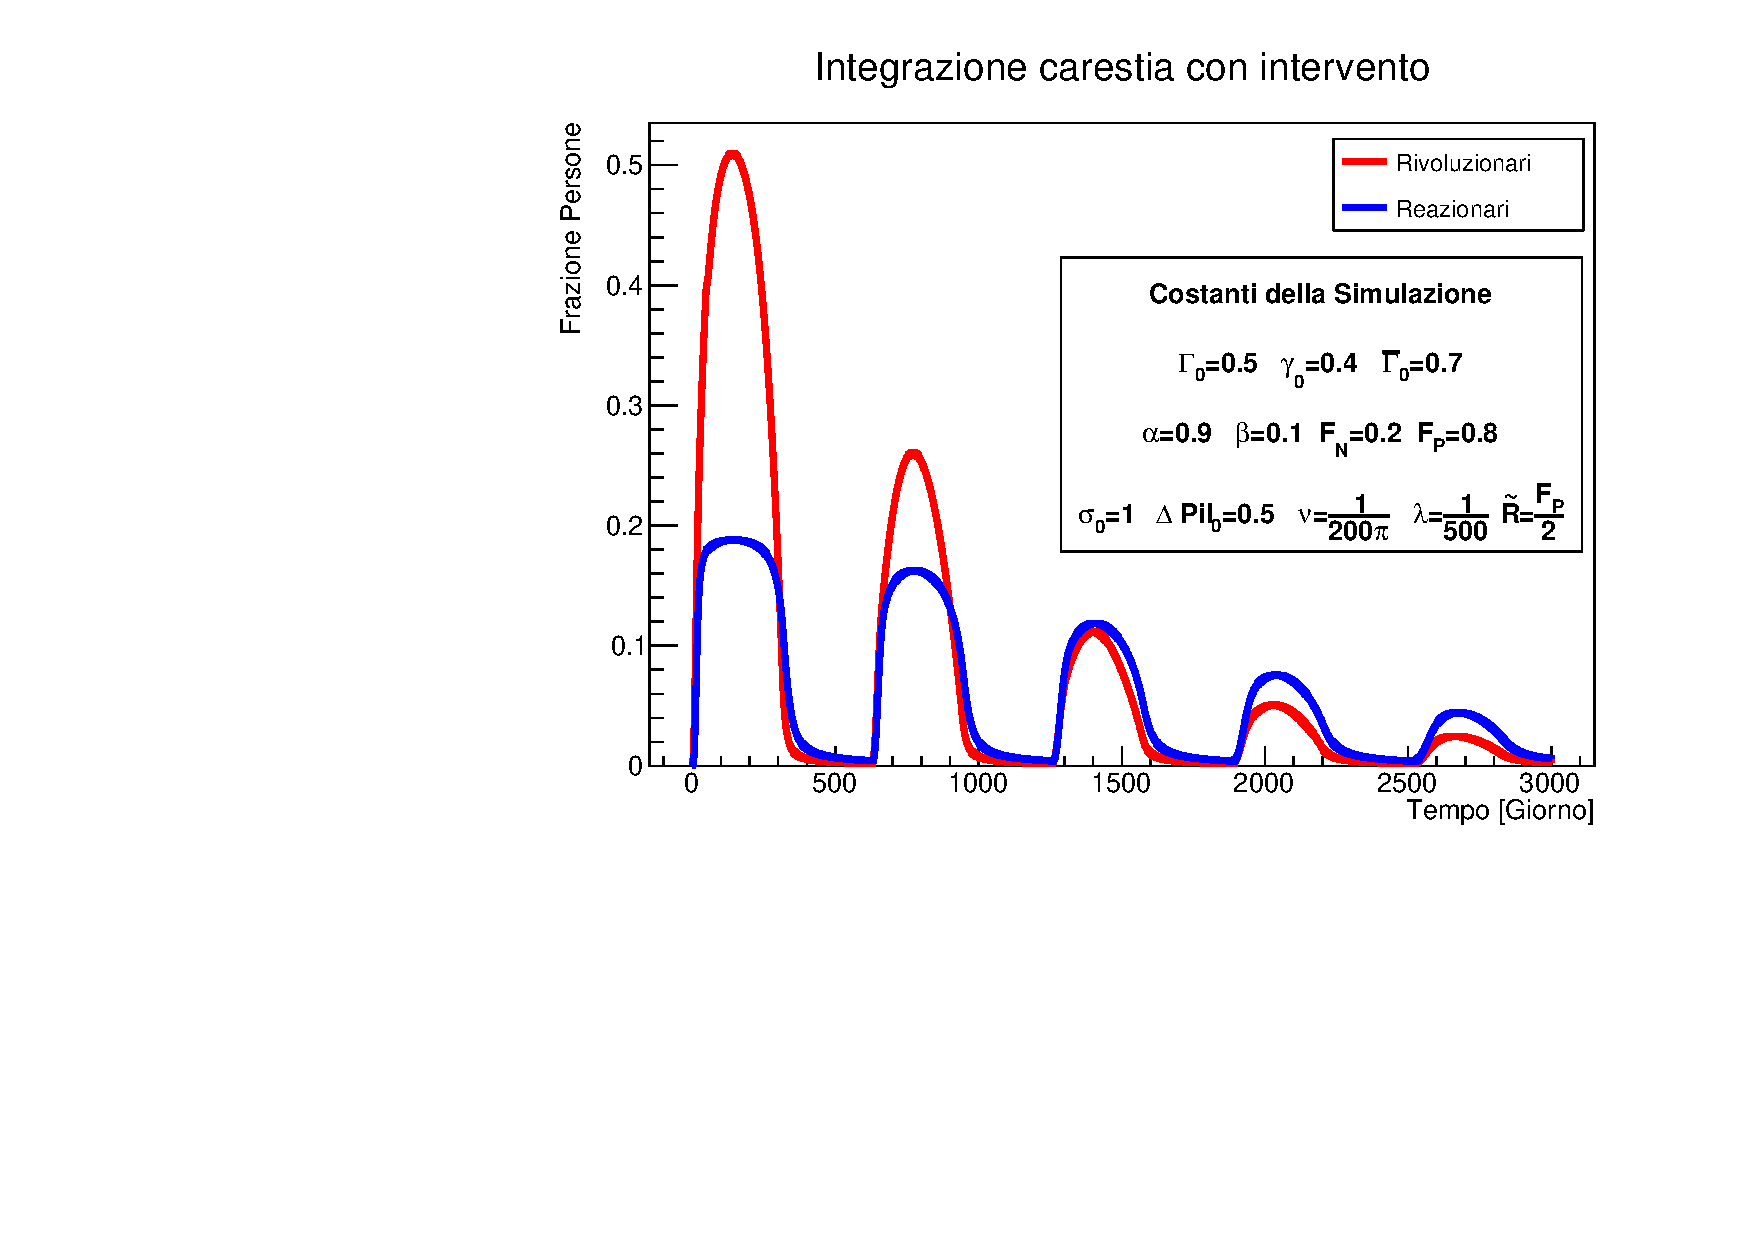
\includegraphics[scale=0.4]{SINEXP.pdf}
	\caption{Integrazione del modello con simulazione di interventi esterni e cartestie.}
\end{figure}
In quest'ultimo caso abbiamo simulato una combinazione dei casi precedenti che risulta a nostro parere essere il caso più realistico. Infatti in questa simulazione si susseguono una serie di carestie che si cerca di mitigare con interventi esterni. In questo caso quello che abbiamo osservato è che le prime rivolte scoppiano e vedono una grande partecipazione da parte dei poveri mentre man mano che la situazione viene mitigata queste rivolte divengono di entità minore fino al punto in cui risultano facilmente controllabili dalla forza a disposizione dei reazionari.
%NOTA:Le funzioni vanno modificate tenendo conto del mezzo seno positivo
\end{itemize}
\newpage
\section{Conclusioni}
Abbiamo studiato la dinamica di una popolazione composta da soggetti poveri e soggetti nobili in grado di insorgere, divenendo rispettivamente rivoluzionari e reazionari, usando un modello multicompartimentale.\\ Dopo aver ipotizzato la forma delle equazioni che descrivono il nostro sistema abbiamo eseguito uno studio dei punti di equilibrio che ci ha permesso di determinare l'esistenza certa di almeno un punto di equilibrio.\\ Abbiamo quindi eseguito l'integrazione numerica delle equazioni e simulato, tramite automa cellulare, il nostro sistema per verificare quanto fosse in grado di rappresentare un dinamica di interazione. Dal confronto tra i grafici abbiamo osservato che, specialmente nella parte transiente, c'è accordo tra i risultati ottenuti con i due metodi. Abbiamo una lieve discrepanza nella fase costante dovuta probabilmente alla natura stocastica della simulazione che porta a fluttuazioni attorno al punto di equilibrio.\\ Abbiamo inoltre  reso variabili nel tempo alcuni parametri, rendendoli dipendenti dalla differenza di reddito e dal rapporto tra le frazioni di popolazione. Descrivendo l'andamento della differenza di reddito in tre modi diversi abbiamo ottenuto tre andamenti che seguono ciò che ci aspettavamo, ovvero un aumento e una diminuzione periodici nel primo caso, un  picco con rapida decrescita nel secondo e infine nel terzo uno sviluppo periodico smorzato, che a nostro parere riflette anche una situazione più realistica.\\ In ogni integrazione emerge chiaramente il carattere di interazione, infatti si osserva una decrescita della componente rivoluzionaria sempre in reazione all'intervento di quella reazionaria. In ogni situazione abbiamo osservato che, più che i valori dei parametri, a fare la differenza sono le frazioni di popolazione. Infatti, utilizzando dei dati storicamente accurati ($ 98\% $ del totale poveri e $ 2\% $ nobili) abbiamo ottenuto sempre un numero di Rivoluzionari nettamente superiore a quello dei Reazionari. %Non so se è il caso di metterlo ma nel dubbio l'ho inserito, al massimo si toglie
\newpage
\appendix
\section*{Appendice}
\section{Metodo di Runge-Kutta 4}
Per l'integrazione numerica abbiamo usato il metodo Runge-Kutta al quarto ordine, detto così perchè l'errore accumulato totale è dell'ordine di $ \mathcal{O}(h^{4}) $, mentre l'errore locale di troncamento è dell'ordine di $ \mathcal{O}(h^{5}) $. 
In generale, dato il seguente problema:
\begin{equation} 
\frac{dx}{dt}=f(x,t)\qquad x(t_{0})=x_{0}
\end{equation}
dove $ x $ è la funzione che si intende approssimare, scegliendo un intervallo $ h>0 $ e definendo:
\begin{equation} 
	x_{n+1}=x_{n}+\frac{1}{6}(k_{1}+2k_{2}+2k_{3}+k_{4})h \qquad t_{n+1}=t_{n}+h
\end{equation}
per $ 0<n<t_{f}/h $, dove $ t_{f} $ é il tempo finale. Usando:
\begin{equation} 
	\begin{aligned}
	&k_{1}=f(t_{n}, x_{n});\\
	&k_{2}=f(t_{n}+\frac{h}{2}, x_{n}+h\frac{k_{1}}{2});\\
	&k_{3}=f(t_{n}+\frac{h}{2}, x_{n}+h\frac{k_{2}}{2});\\
	&k_{4}=f(t_{n}+h, x_{n}+hk_{3});
\end{aligned}
\end{equation}
Per ogni $ n $, il valore successivo $ x_{n+1} $ da quello attuale $ x_{n} $ e dalla media pesata di quattro incrementi, i quali sono il prodotto dell'intervallo $ h $ e la pendenza data da $ f $. In particolare:
\begin{itemize}
	\item $ k_{1} $ é la pendenza all'inizio dell'intervallo, usando solo $ x $ 
	\item $ k_{2} $ é quella a metà intervallo, usando $ x $ e $ k_{1} $
	\item $ k_{3} $ è di nuovo a metà, ma usando $ x $ e $ k_{2} $
	\item $ k_{4} $ é quella alla fine, usando $ x $ e $ k_{3} $
\end{itemize}
\section{Come ricavare il punto di equilibrio}
Partendo dal sistema:
\begin{equation}
	\begin{cases}
		\Gamma (F_{P}-R)R+\gamma (F_{P}-R)-\bar{\Gamma}R\bar{R}=0\\
		\alpha (F_{N}-\bar{R})R-\beta (F_{P}-R)\bar{R}=0
	\end{cases}
\end{equation}
riscriviamo la seconda equazione come:
\begin{equation} \label{B2}
	R\bar{R}(\beta - \alpha)+R\alpha F_{N}-\beta F_{P}\bar{R}=0
\end{equation}
mentre dalla prima equazione possiamo ricavare $ \bar{R} $ in funzione di $ R $:
\begin{equation}
	\bar{R}=\frac{\Gamma}{\bar{\Gamma}}(F_{P}-R)+\frac{\gamma}{\bar{\Gamma}}\frac{F_{P}-R}{R}
\end{equation}
A questo punto basta sostituire $\bar{R} $ nella \ref{B2} e si ottiene:
\begin{equation}
	R(\beta - \alpha)\left[\frac{\Gamma}{\bar{\Gamma}}(F_{P}-R)+\frac{\gamma}{\bar{\Gamma}}\frac{F_{P}-R}{R}\right]+R\alpha F_{N}-\beta F_{P}\left[\frac{\Gamma}{\bar{\Gamma}}(F_{P}-R)+\frac{\gamma}{\bar{\Gamma}}\frac{F_{P}-R}{R}\right]=0
\end{equation} 
Portando a denominatore comune si ottiene:
\begin{equation}
	R^{3}(\beta - \alpha)\frac{\Gamma}{\bar{\Gamma}}-R^{2}\left(\alpha F_{N}+(\beta - \alpha)\frac{\Gamma}{\bar{\Gamma}}F_{P}-(\beta - \alpha)\frac{\gamma}{\bar{\Gamma}}+\beta F_{P}\frac{\Gamma}{\bar{\Gamma}}\right)-\frac{R}{\bar{\Gamma}}\left(\gamma (\beta - \alpha)F_{P}-\beta \Gamma F^{2}_{P}+\gamma\beta F_{P}\right)+\frac{\gamma\beta}{\bar{\Gamma}}F^{2}_{P}=0
\end{equation}
Risolvendo questo polinomio di terzo grado possiamo ricavare i punti di equilibrio.